\chapter{Introduction}
\label{chp:introduction}

The foundation of science is based on experiments.
This understanding of today's science was introduced by Sir Isaac Newton in his revolutionary work \emph{hilosophiae naturalis principia mathematica}.
Newton reasoned that researchers are to test their hypothesis with observable, measurable and empirical experiments.
To this day, this approach is applied by many researchers.
Especially in the area of Computer Science, it is key to provide empirical proof that a hypothesis one ought to prove holds.
This empirical proof often manifests itself in the form of benchmarking.
By comparing several programs or different versions of the same program on a variety of workloads, researchers can determine the performance.

In this thesis we introduce a performance regression testing system for IO that makes use of benchmarking.
Whenever a codebase changes, it is important to measure the effects of these changes.
Negative changes can manifest themselves as reduced computational speed, increased memory consumption or reduced responsiveness of a program.
Each of these result in a reduction of user experience.
For instance, Google Chrome makes use of performance regression testing to gain insight into the effect of code changes.
While it is one of the fastest browsers currently available, it is also know for it's extreme RAM consumption which may lead to issues on older devices.

Over the course of years, profilers have been introduced to allow developers to profile their running code.
By inspecting the data generated by these profilers, developers can pinpoint functions that are consuming e.g. a lot of wall- or CPU time which may indicate a bottleneck is present.
Additionally, once a bottleneck has been resolved it can be verified by using a profiler that it indeed does consume less resources, i.e. time or memory.

However, in large and complex systems there are likely to be many bottlenecks present.
J. M. Juran's Pareto principle admonishes that one should "Concentrate on the vital few, not the trivial many". This principle is also known as the 80/20 rule \cite{ammons2004finding}.
Concretely, this means that resolving the vital bottlenecks yields the best diminishing returns.
This principle holds even for large systems.

In this thesis we use the BitTorrent client Tribler as a use case to implement a regression testing system and to find and resolve bottlenecks demonstrating the working of said system.
Tribler has been in development for over ten years and has grown into a highly complex and large distributed system.
Tribler along with its components features more than 158 KLOC \cite{tribler2015about}.
The remainder of this chapter is used to introduce Tribler and its components as well as providing the outline of this thesis.

\section{Tribler}
Tribler is a research platform for self organizing systems and online cooperation.
Currently, this work is embedded in the Tribler BitTorrent client, visible in Figure X \todo{Add screenshot of 6.5}.
It has been downloaded approximately 1.8 million times, has more than 2 thousand monthly active users and anticipating more growth in the near future.\todo{Cite Pouwelse's slides.}.

Tribler focuses on the following goals:
\begin{itemize}
    \item Allow for secure and private communication and sharing of data.
    \item Enforce user contribution in the network by making use of the Multi-Chain.
    \item Reward seeding of poorly-seeded content by using credit mining.
    \item Make it impossible to shut Tribler down, unless the Internet itself as a whole gets taken down.
\end{itemize}

A fully decentralized ecosystem i.e. no central components present, is Tribler's approach to achieve these goals.
Tribler has been designed and build with this focus~\cite{Pouwelse-tribler,Bakker-tribler}.
A distributed network requires both the presence and collaboration of participants, called peers, to be able to achieve this.

% \begin{figure}
%	\centerline{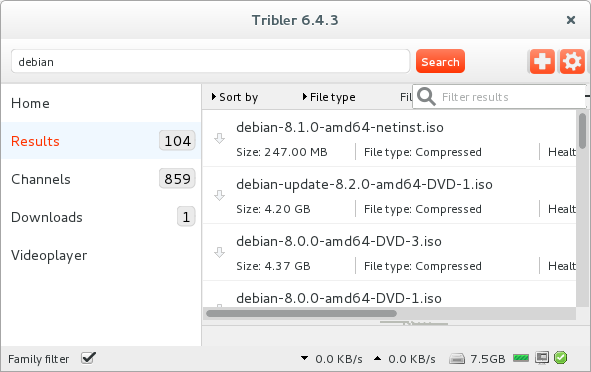
\includegraphics[scale=0.6]{introduction/figs/tribler-screenshot.png}}
%	\caption{Screenshot of Tribler v6.4.3.}
%	\label{fig:tribler-screenshot}
%\end{figure}

\section{Dispersy}
The Distributed Permission System (Dispersy) is an elastic database system written in the Python programming language and uses SQLite as its underlying database engine.
It is designed to still function when faced with challenging network conditions such as low internet speed, connection drops, package loss and even when hurdles such as firewalls are in place.
Additionally, Dispersy is built to scale very well; it can handles communication with thousands of peers simultaneously.
It workings have been proven throughout the years as it's heavily used within the Tribler client and is maintained by the Tribler organisation.

In Dispersy one can define communities in which peers can send messages to each other.
Every community and peer is uniquely identified and secured by making use of elliptic curve cryptography.
By performing peer exchanges (PEX) and by making use of Distributed Hash Tables (DHT's), peers receive continuously information about the network.

One of Dispersy's unique points is that it does not rely on a central component with the exception of bootstrap servers.
Furthermore, Dispersy's main features are:
\begin{itemize}
	\item Stateless synchronization using Bloomfilters.
	\item Decentralized NAT traversal.
	\item Performance that can scale to over 100,000 bundles.
\end{itemize}

\section{BitTorrent protocol}
The BitTorrent protocol was introduced in 2001 and been a huge part of the internet ever since \cite{Cohen2001BitTorrent}.
Estimates as of 2009 indicate that 43\% to 70\% of all internet traffic world-wide is caused by peer-to-peer networks \cite{schulze2009internet}.
As of February 2013, BitTorrent was responsible for 3.35\% of all worldwide bandwidth \cite{palo2013application}, having 15 - 27 million concurrent users at any time \cite{wang2013measuring} and more than 150 million users in total \cite{reuters2012bittorrent}.

Downloading files is done in a decentralized way, that means no central entity such as a server is needed.
By obtaining a torrent file, users can download files associated with this torrent using a program that is compatible with the BitTorrent protocol.\\

A torrent is a file that contains information about the files and \todo{add how a torrent file works, what it contains and how you are downloading e.g. connecting to peers.}\\

When sharing files by using the BitTorrent protocol, a user (or peer) that uploads i.e. provides a file to the BitTorrent network, is called a seeder.
A peer that is downloading a file of a seeder is called a leecher.
Any peer can be both a seeder and leecher at the same time, and join the network at any given time.\\

The ratio between the total data downloaded and uploaded is called the seeding ratio \cite{Cohen-bittorrent}.
The seeding ratio can be seen as an indication of the level of collaboration i.e. giving back resources to the network.\\

%Seeding can be seen as an interaction between peers, where the seeder aids the leeching peer.
%By utilizing the seeders upload bandwidth, the leeching peer can use his download bandwidth to download a file.
%While there is a clear incentive for the leecher by downloading the desired file, there is none for the seeder.
%Especially since the leecher has a little chance of becoming also be a seeder for the original seeder \cite{Lai-Incentives}.\\

%Having peers actively and persistently contribute to the network will increase the network's health which in turn provides several benefits for all peers.
%A more healthy network results in a higher availability of seeders and results in high download speeds.
%It has been shown that private communities i.e. "darknets" where the seeding ratio is high, provides better download conditions \cite{meulpolder-privatecommunities}.
%In these private communities, trackers i.e. central components introduce peers to each other using the Tit-for-tat approach \cite{cohen-titfortat}.
%The Tit-for-Tat approach is aiding peers who have aided you in the past,
%The absence of trackers, which is often the case in public networks, results in free-riding \cite{Adar-Freeriding}.
%A free-riding peer does not or gives little back to the network while receiving all benefits i.e. download without any restriction.
%\todo{Explain the optimistic chocking approach.}
%BitTorrent applies a variation of the Tit-for-tat strategy, optimistic chocking, to combat this problem.
%The Tit-for-Tat strategy is to only provide help to peers that return this help.
%However, it has been shown that this approach is not effective in battling abuse \cite{Pouwelse-tribler}.

\section{Asynchronous programming}
\label{sec:async-programming}

When programming asynchronously the function that is being called (callee) by a caller returns a so-called deferred.
A deferred is a place holder for the actual value that this function will return once the callee has computed it.
In normal (synchronous) programming, when calling a function the caller is waiting for the callee to provide an answer. 
Making a synchronous call in a single or multi-threaded environment may not be efficient.
If the callee takes a long time to compute and return the answer, the caller thread will be idle for that duration.
When using deferreds, the callee will simply return a Deferred and starts the computation.
The caller will resume its other operations and when the callee is done, it will fire a callback event, notifying that the deferred has either resolved into an answer or an error.
By attaching a callback and an errback, the caller can handle the case of a success and failure respectively.\\

One of the dangers of asynchronous programming is that during the callee's computation, the caller will also continue.
This may result in the caller changing values, the callee is dependent on.


\todo{more explanation needed.}
\section{Outline}
In this chapter we provided an introduction of this thesis and presented the research questions this thesis aims to answer. 
This section describes the other chapters in this thesis and their relevance to the research questions provided in section \ref{chp1:sct:objectives-research-questions}.
Chapter \ref{chp:preliminaries} provides preliminaries and terminology used through this thesis.
Chapter \ref{chp:problem-description} presents an overview of some of the problems Tribler is currently facing which this thesis addresses.
Chapter 
\todo{Add more here as cahpters are added.}
